\subsection{Exam: 2022. 05. 30., Exercise 3}

\label{exam_2022_05_30_exercise_3}

\lineparagraph{Exercise}

Consider the following decision problem. We are given an undirected connected
graph $G$ of even number of vertices, whose edges are colored red or blue.
We want to decide whether there exists a Hamiltonian cycle in $G$ that consists
of a red path and a blue path ofthe same length, that is, going along the
Hamiltonian cycle, the red edges form a path and the blue edges form a path
and those two paths have the same number of vertices. Prove that this problem
is NP-complete.

\lineparagraph{Solution}

I belive this exercise caused the most problems and misunderstandings on the exam,
so let's break down and understand what we are being asked for here.

\begin{itemize}
\item We are given decision problem, let's name its language $HAMRB$, for Hamiltonian-cycle, red-blue version.
\item The input is a graph here, which already has its edges colored in for us in red and blue colors. The coloring is given, we cannot modify this. (Many students did try to color the edges.)
\item We are asked the question, whether there is a Hamiltonian-cycle (a cycle that contains all vertices of the graph) in this graph, which has a ''red edged half'' and a ''blue edged half'', like so:

\begin{center}
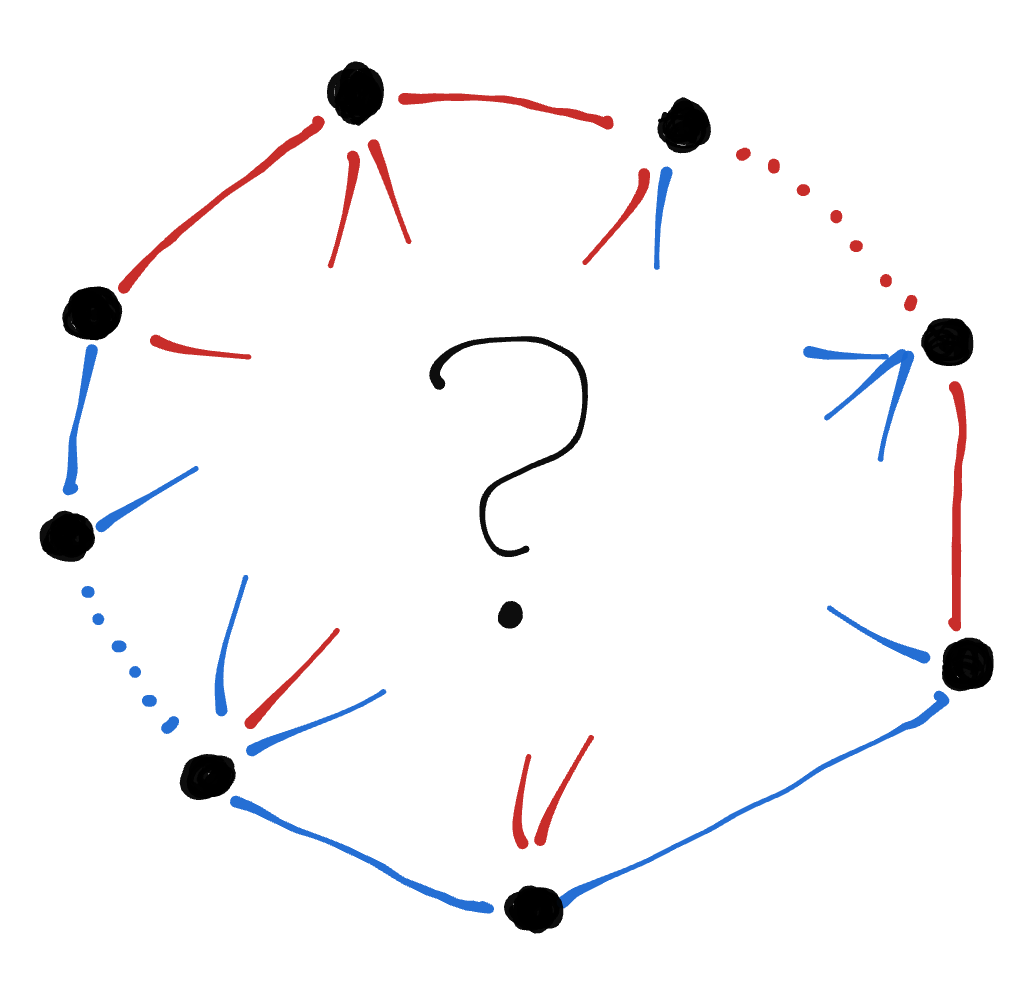
\includegraphics[width=0.7\linewidth]{./exams/2022_05_30/03/hamrb.png}
\end{center}

\item It is easy to see this structure in the graph now, because the vertices are laid out or us in a nice way, in the correct order, however when you are given a graph, it is difficult (we'll prove soon that it's NP-complete :) ) to find this special cycle.
\item In order to show that this problem is NP-complete, we must show that it is both in NP and NP-hard.
\end{itemize}

\textbf{Step 1: Showing that HAMRB }$\mathbf{\in{}}$\textbf{ NP}

\begin{itemize}
    \item To show that a language is in NP, we use the Witness Theorem.
    \item To use the Witness Theorem, we have to give the following things for $HAMRB$:
    \begin{itemize}
        \item A witness:
            \item A witness must exist for every input in $HAMRB$, every colored edged graph, which has this type of red-blue Hamiltonian-cycle in it.
            \item A witness like this cannot exist for any input that is not in $HAMRB$, so if it does not have type of red-blue Hamiltonian-cycle in it.
            \item The size of the witness must be polynomial in relation to the input size.
        \item A witness checking algorithm:
            \item Must be able to verify, that the witness is correct. We do not trust the person that gives us the witness, but based on the witness we can check whether the input is in $HAMRB$ or not.
            \item Usually the witness is basically the ''solution'' of the problem, think of how solving a Sudoku-puzzle is difficult, but if someone fills out a Sudoku table for us, it is easy to verify if the solution is correct. In this case the witness is the filled-out Sudoku-table, while the input is the initial table.
            \item This must run in polynomial time relative to the input and witness size.
    \end{itemize}
    \item In this case, the witness (the solution to the problem) is going to be the list of all of the vertices of the graph, in the order in which they are present in the cycle. E.g. $\{v_1,v_2,\dots{}v_n\}$. And the starting vertex should be the first red edge, so it's easier to check.
    \item Given this ordering, we can verify that this is indeed a correct solution, since we can check the following:
    \begin{itemize}
        \item All vertices of the graph are present.
        \item All cycle edges exist, so there is an edge between vertices $v_1$ and $v_2$, between $v_2$ and $v_3$, between $v_3$ and $v_4$, and so on, $v_{n-1}$ and $v_n$ and finally $v_n$ and $v_1$.
        \item The first half of the checked edges above are red, the second half of the checked edges above are blue.
    \end{itemize}
    \item The witness' size is $O(n\log_{2}n)$, since there are $n$ vertices and one of them can be represented by its index, so a number in a binary format, that requires $log_{2}n$ bits. This is polynomial relative to the $O(n^2)$ input size (adjacency matrix with coloring information).
    \item The witness checking algorithm did a for loop on all vertices 3 times, which makes it polynomial.
\end{itemize}

\textbf{Step 2: Showing that HAMRB is NP-hard}

\begin{itemize}
    \item In order to sho that $HAMRB$ is NP-hard, we have to Karp-reduce another NP-hard (NP-complete) language onto it. Please read Section \ref{karpwhat}, \nameref{karpwhat} to understand what a Karp-reduction is and continue with the next item after you're done.
    \item What's happening now is this: in order to show that $HAMRB$ is a difficult problem to solve, we are going to show, that if we had a solution to $HAMRB$, then we could use that algorithm to solve another well-known difficult problem. So the solution to $HAMRB$ is also a 'big achievement' to figure out.
    \item The hardest part here is figuring out which well-known difficult problem could be solved with the $HAMRB$ solver.
\end{itemize}

\begin{center}
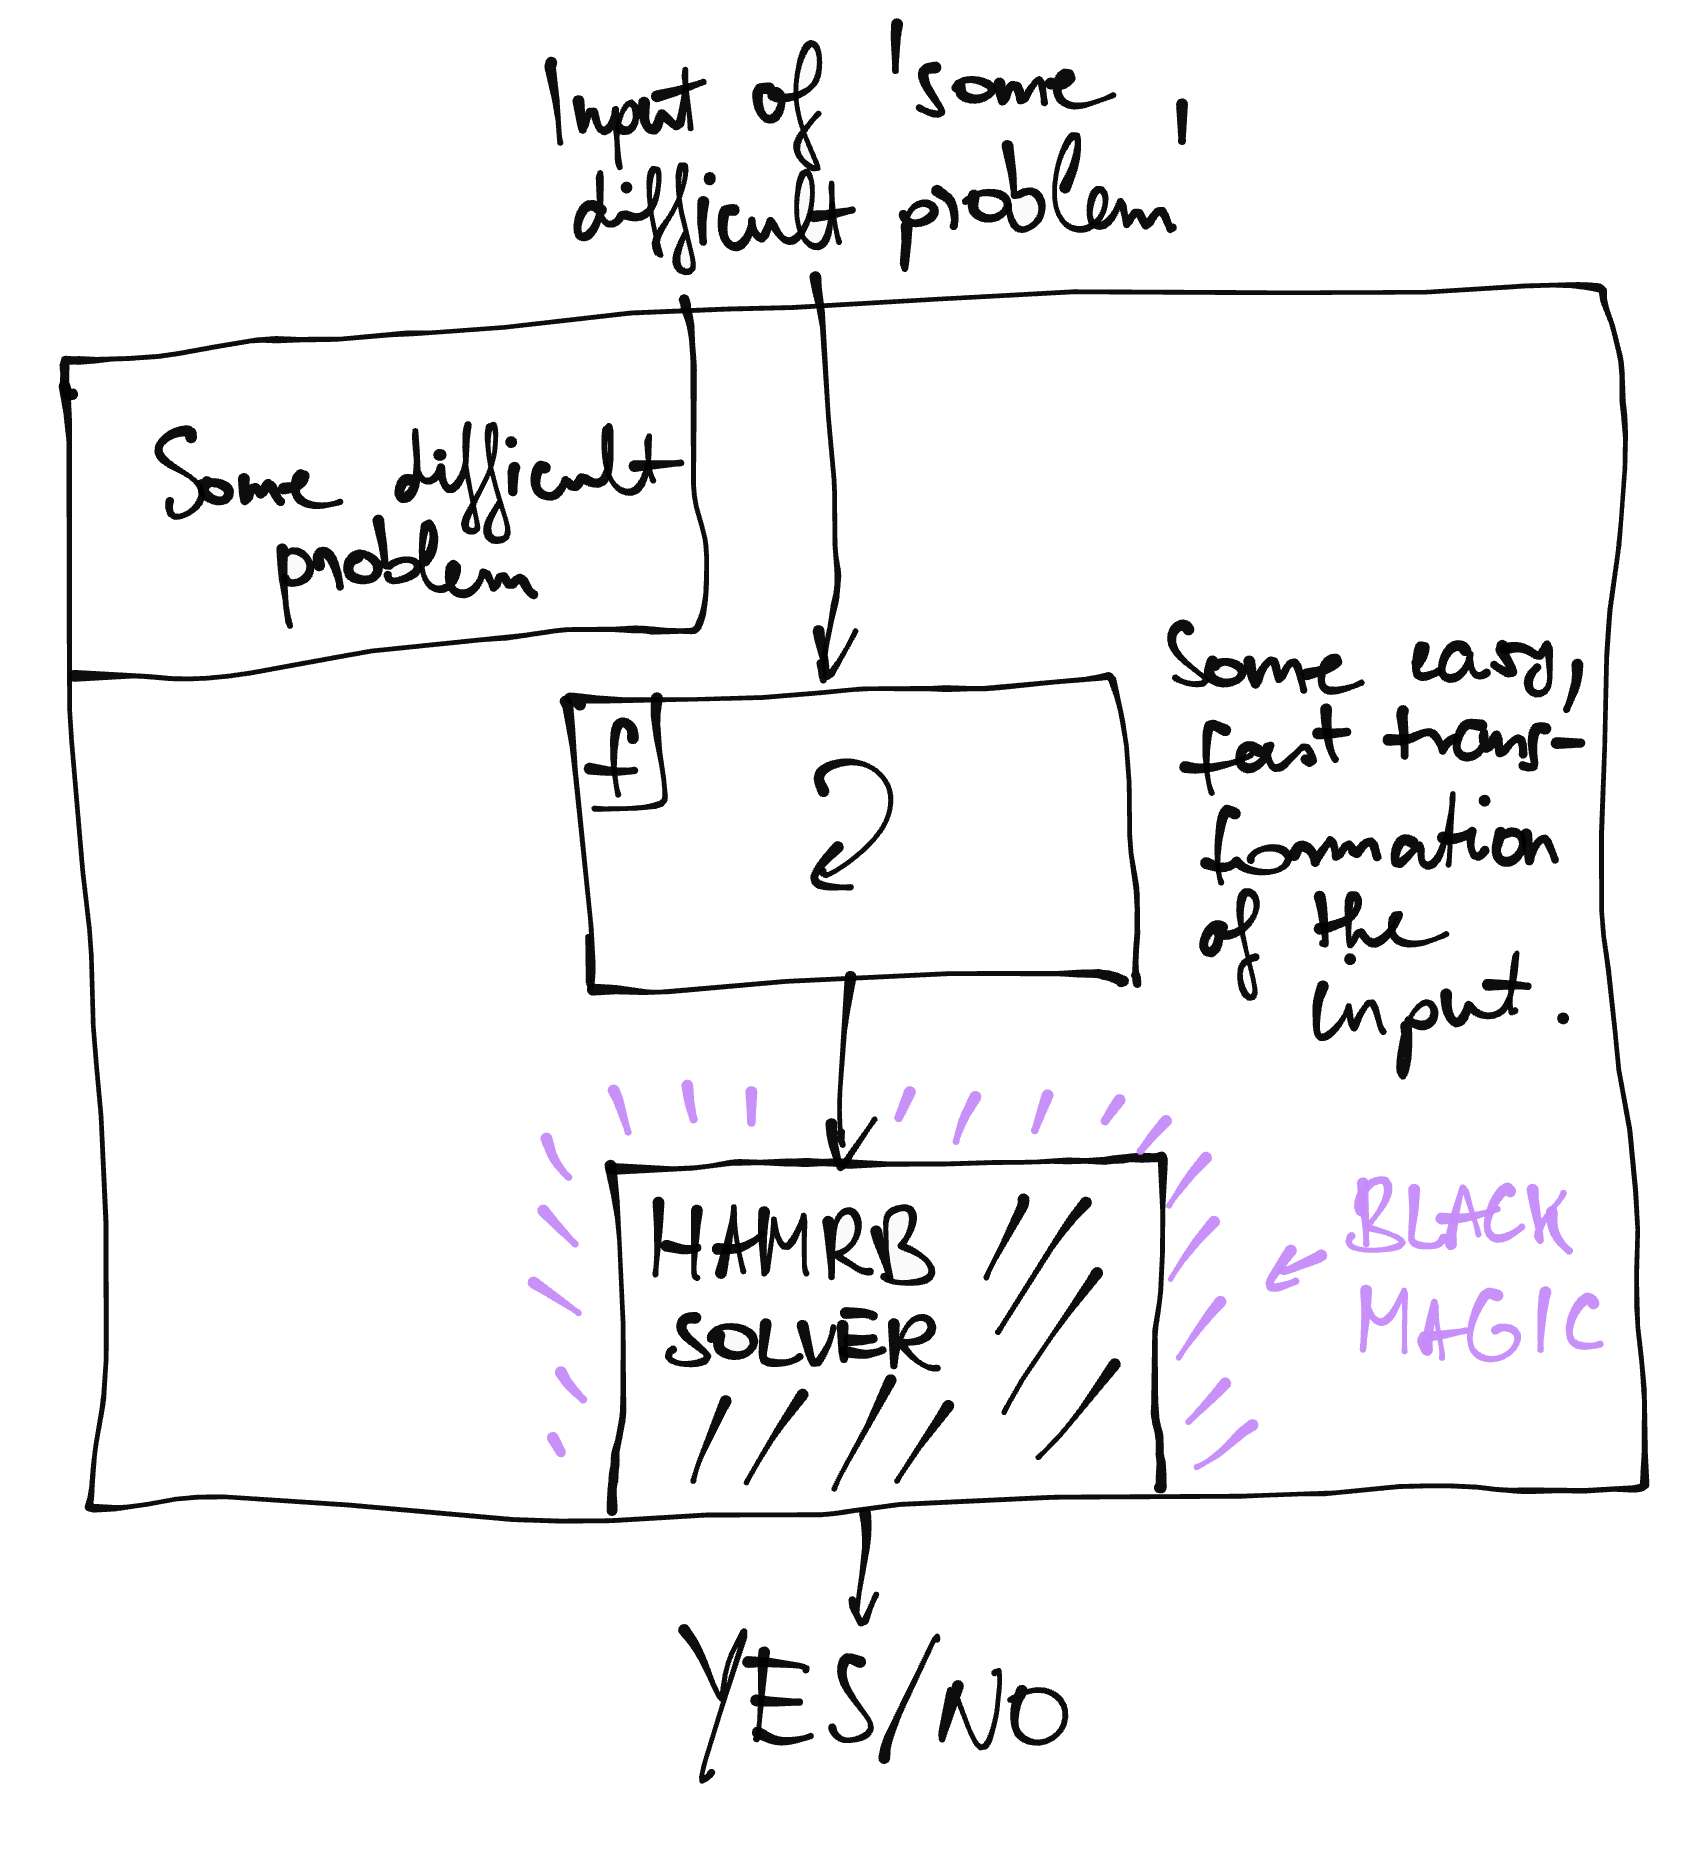
\includegraphics[width=0.9\linewidth]{./exams/2022_05_30/03/hamrb_karp.png}
\end{center}

\begin{itemize}
    \item Luckily, we have only studied a few of these problems, namely (I'm giving the decision version of the problems, which can all be turned into optimization problems):
    
\end{itemize}
\begin{center}
\begin{tabular}{|l|l|}
\hline
\makecell[l]{SAT($\Phi$)} & \makecell[l]{Given the $\Phi$ boolean formula, can it be\\ satisfied, e.g. is there an assigment of the variables in it\\ for which the formula evaluates to true?} \\
\hline
\makecell[l]{3-SAT($\Phi$),\\4-SAT($\Phi$),\\\dots{},\\n-SAT($\Phi$), where $n\geq{}3$} & \makecell[l]{Given a ($\Phi$) formula of Boolean-variables,\\ which is specifically in \href{https://en.wikipedia.org/wiki/Conjunctive_normal_form}{conjunctive normal form},\\ where a term consists of exactly $n$ variables,\\ can this formula be satisfied?\\ Be careful, 2-SAT is in P!} \\
\hline
\hline
\makecell[l]{MAXINDEP(G, k)} & \makecell[l]{Is there a set of independent vertices of size (at least) $k$ in $G$?} \\
\hline
\makecell[l]{MAXCLIQUE(G, k)} & \makecell[l]{Is there clique of size (at least) $k$ in $G$?} \\
\hline
\makecell[l]{3-COLOR(G),\\4-COLOR(G),\\\dots{},\\n-COLOR(G), where $n\geq{}3$} & \makecell[l]{Can $G$'s vertices be properly colored using $3$\\ colors? (So no two vertices of the same\\ color have an edge running between them.)\\ Be careful, 2-COLOR is in P!} \\
\hline
\makecell[l]{HAM(G)} & \makecell[l]{Does graph $G$ contain a Hamiltonian cycle\\(a cycle that contains all vertices of $G$)?} \\
\hline
\makecell[l]{HAMPATH(G)} & \makecell[l]{Does graph $G$ contain a Hamiltonian path\\(a path that contains all vertices of $G$)?} \\
\hline
\makecell[l]{s-t-HAMPATH(G, s, t)} & \makecell[l]{Does graph $G$ contain a Hamiltonian path that\\starts specifically in vertex $s$ and ends in vertex $t$?} \\
\hline
\makecell[l]{TSP(G, n)} & \makecell[l]{Given a complete weighted graph $G$ (distances of cities),\\is there a Hamiltonian cycle with a weight of at most $n$?} \\
\hline
\hline
\makecell[l]{SUBSETSUM($a_1, a_2, \dots{} a_n, t$)} & \makecell[l]{Is there a subset of the integers $a_1,\dots{}a_n$\\that sum to exactly $t$?} \\
\hline
\makecell[l]{PARTITION($a_1, a_2, \dots{} a_n$)} & \makecell[l]{Can you partition the integers $a_1,\dots{}a_n$\\into exactly two sets, such that their sum is equal?} \\
\hline
\hline
\makecell[l]{IP($A,b,c^T,k$)} & \makecell[l]{Integer programming:\\Is there an $x$ integer vector for which $k\leq{}c^Tx$, while $Ax\leq{}b$?\\Be careful, LP (linear programming) is in P!} \\
\hline
\hline
\makecell[l]{BINPACKING($s_1,s_2,\dots{}s_n,k$)} & \makecell[l]{Can we place all of the $s_i$ items of size $0\leq{}s_i\leq{}1$\\ into at most $k$ number of size $1$ bins?} \\
\hline
\makecell[l]{KNAPSACK($s_1,s_2,\dots{}s_n,v_1,v_2,\dots{}v_n,S,V$)} & \makecell[l]{Can we select a subset of the items $i$, so that\\ their size $s_i$ sums to at most $S$,\\while their value $v_i$ sums to at least $V$?} \\
\hline
\end{tabular}
\end{center}

\begin{itemize}
    \item The task here is to select one from the above and try to transform its input into something that we can give to $HAMRB$ and whenever $HAMRB$ returns yes, that means that the answer to the original problem is also yes, and same for no.
    \item It is a good idea to start looking around the problems that are similar to the one being asked at first, and when we have no success, then try to move onto different ones.
    \item In this case HAM, HAMPATH and s-t-HAMPATH are the ones that are similar.
    \item Many students have tried to use HAM here, but I believe that one would be more tricky to figure out (remember, if one of them can be Karp-reducted, then all Karp-reductions exist, all NP-complete languages can be Karp-reduced to all others, however some of them are harder to figure out (or can be done indirectly)!).
    \item I believe the best choice here is s-t-HAMPATH, because the $s$ and $t$ vertices are fixed, which will make it easier for us to define a coloring of the transformed graph's edges (you'll see why)!
    \item So the Karp-reduction we are doing is $s-t-HAMPATH \prec HAMRB$:
\end{itemize}

\begin{center}
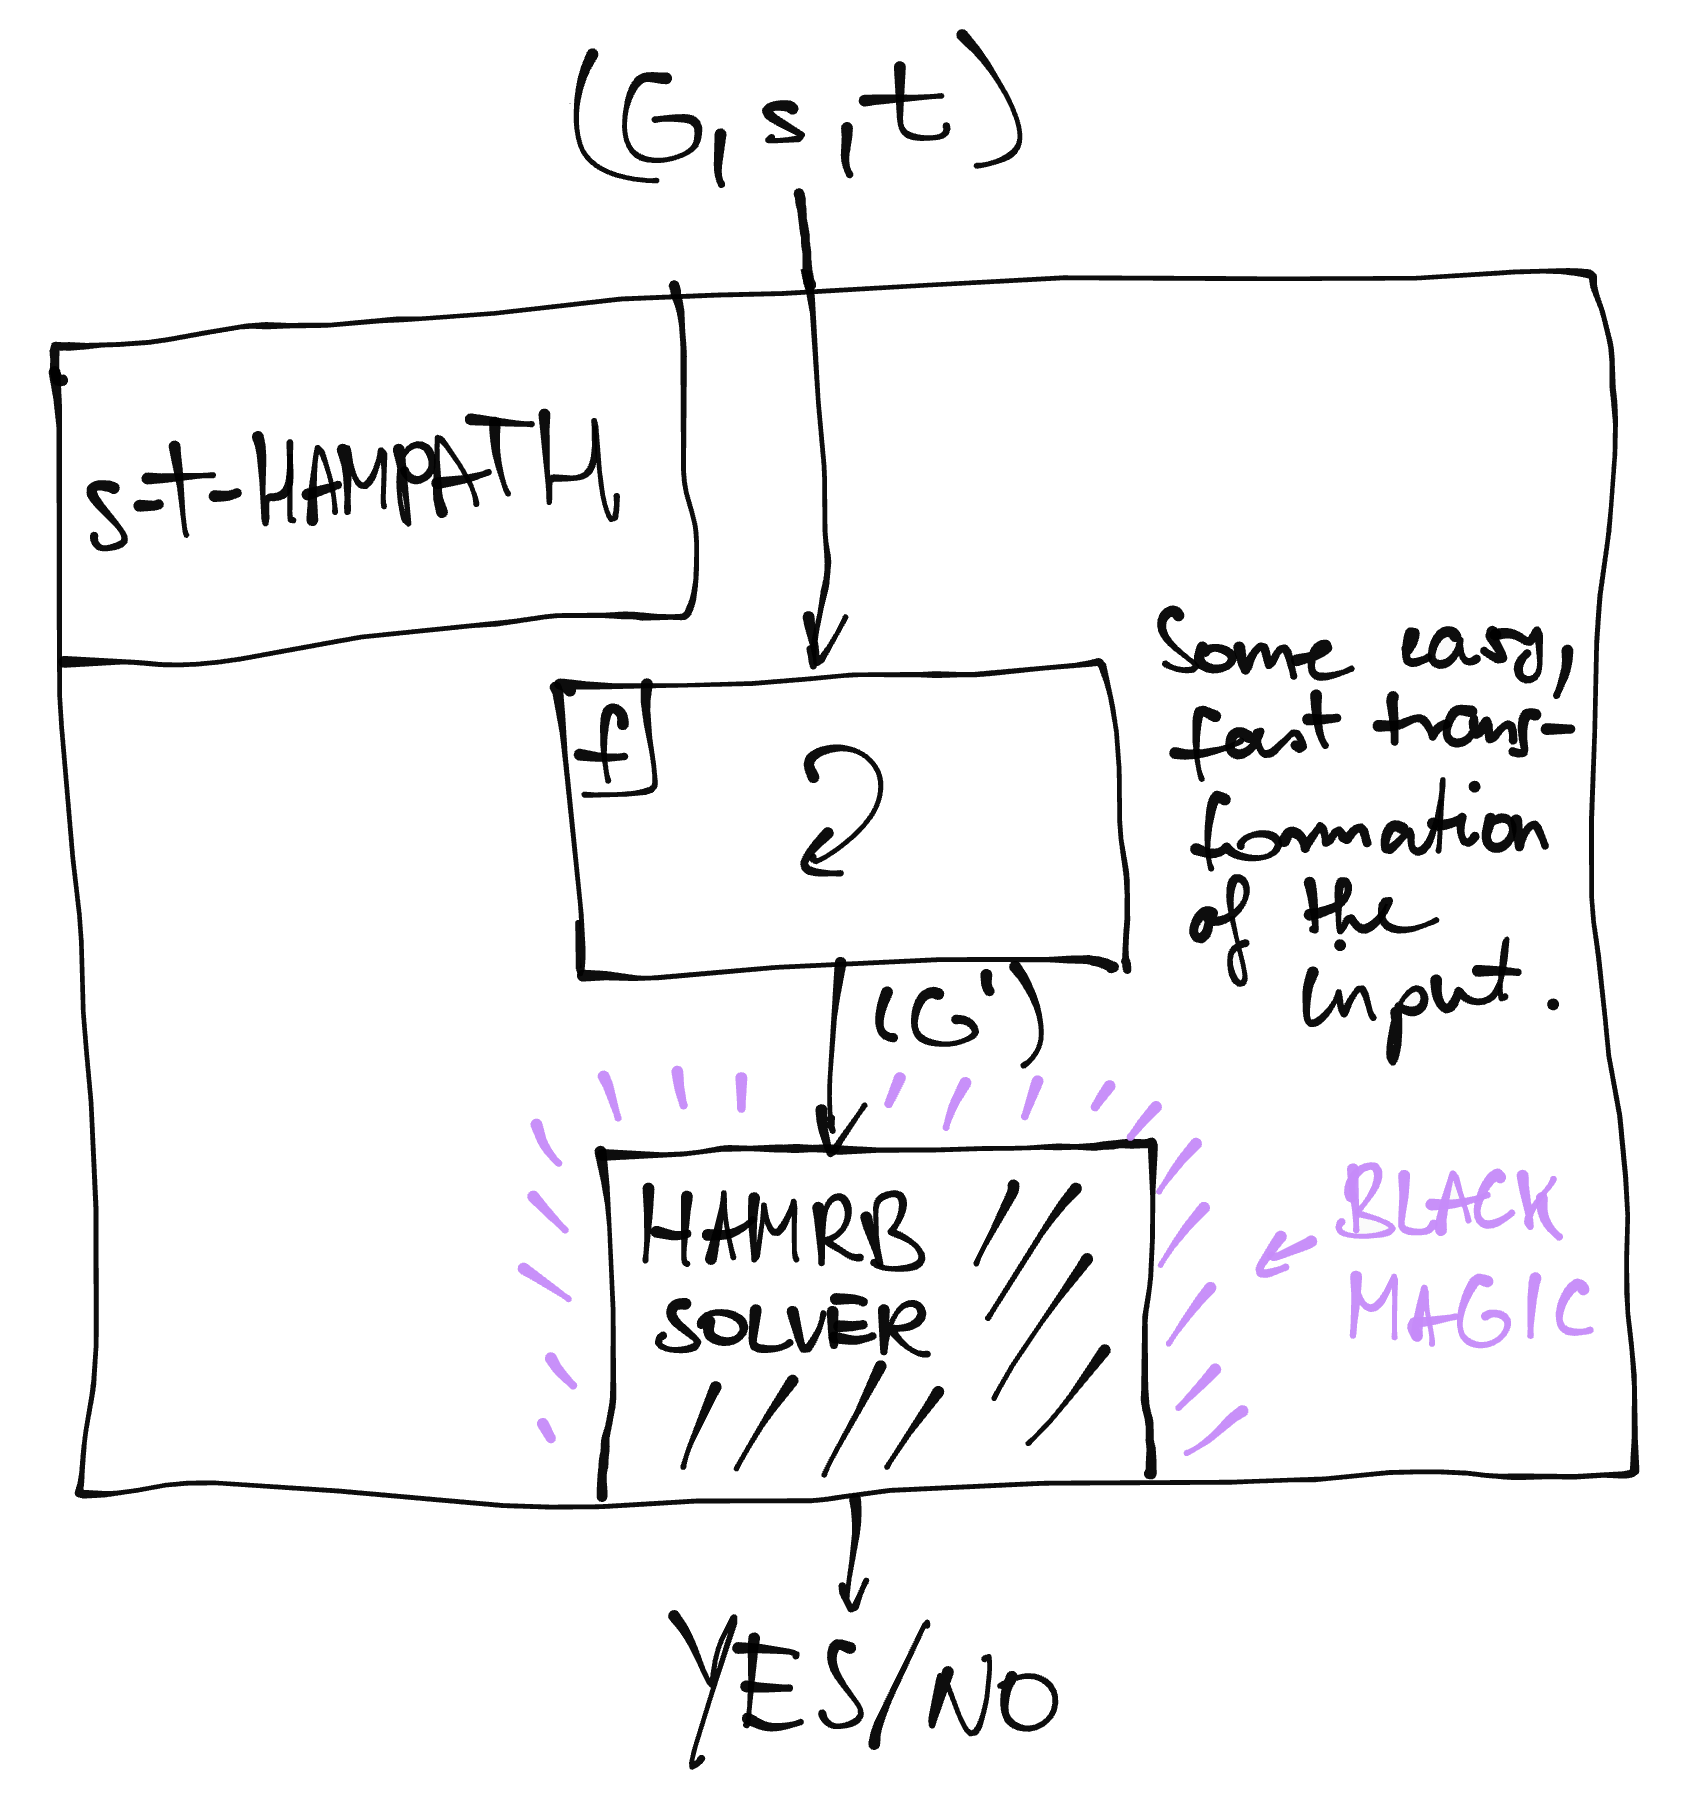
\includegraphics[width=0.9\linewidth]{./exams/2022_05_30/03/sthampath_hamrb_karp.png}
\end{center}

\begin{itemize}
    \item Now we need to figure out what $f$ is.
    \item The biggest problem I saw here in the exam papers is that many students thought that we know where the s-t-HAMPATH (or in the case of $HAM \prec HAMRB$, where the Hamiltonian-cycle) is. This is an incorrect assumption, we do \textbf{not} know where the s-t-HAMPATH is in $G$! We need to figure out if it exists or not, using the ''blackbox'' solution to $HAMRB$. We will transform the input $(G,s,t)$ into a $G'$ graph, which has a red-blue-Hamiltonian cycle exactly when $G$ has an s-t-HAMPATH.
    \item How do we do this:
    \item While we do not know where the full s-t-HAMPATH is going, we do know the first and last vertex on it, $s$ and $t$.
    \item We begin with the input we receive for s-t-HAMPATH: $(G,s,t)$:
\end{itemize}

\begin{center}
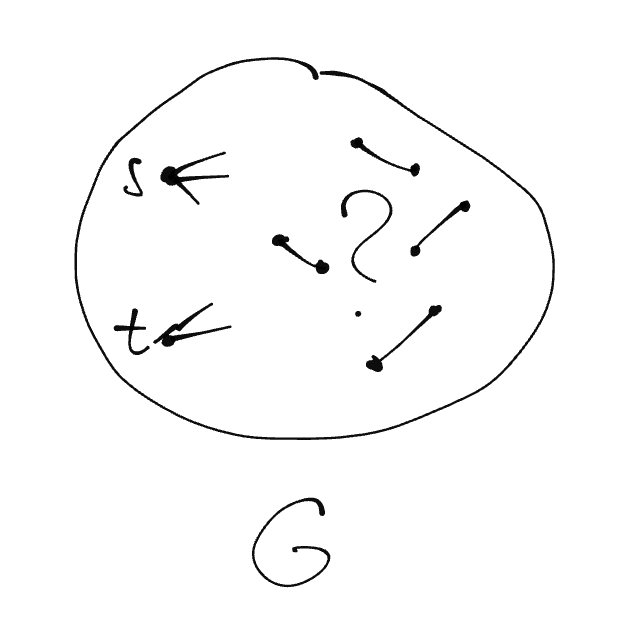
\includegraphics[width=0.4\linewidth]{./exams/2022_05_30/03/karp_0.png}
\end{center}

\begin{itemize}
    \item We are going to create a copy of G, like so:
\end{itemize}

\begin{center}
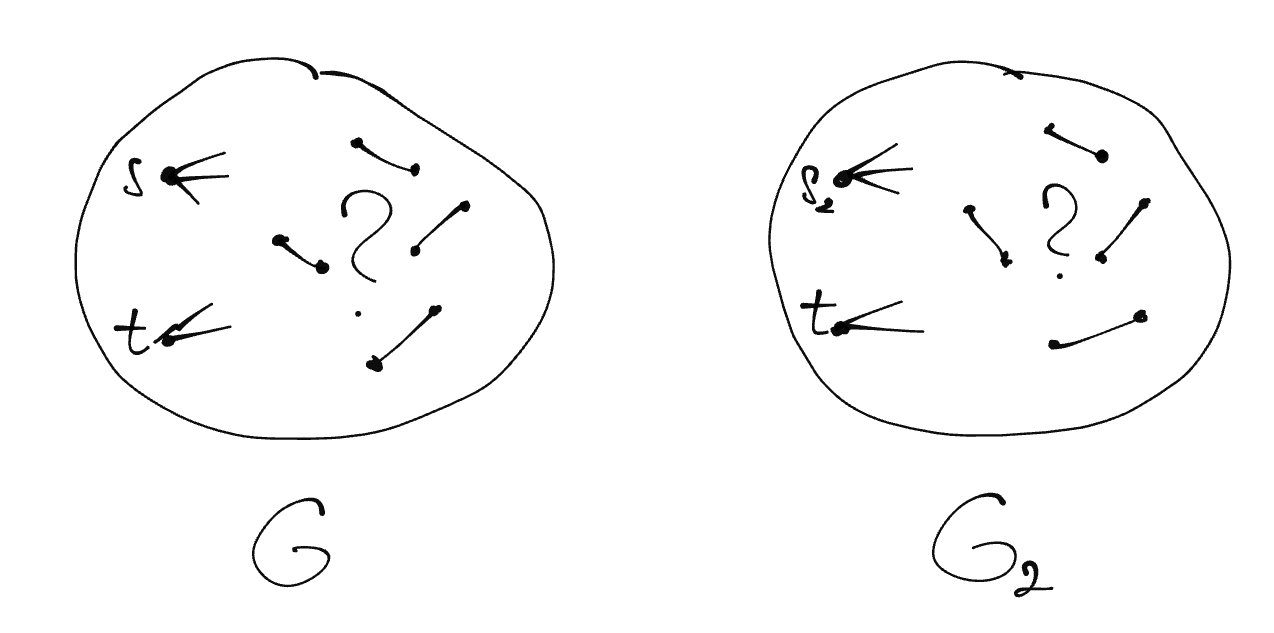
\includegraphics[width=0.9\linewidth]{./exams/2022_05_30/03/karp_1.png}
\end{center}

\begin{itemize}
    \item Now we will color all of the edges in $G$ red and all of the edges in $G_2$ blue. \color{red}{\textbf{Notice here how we don't need to know where the HAMPATH is!}}
\end{itemize}

\begin{center}
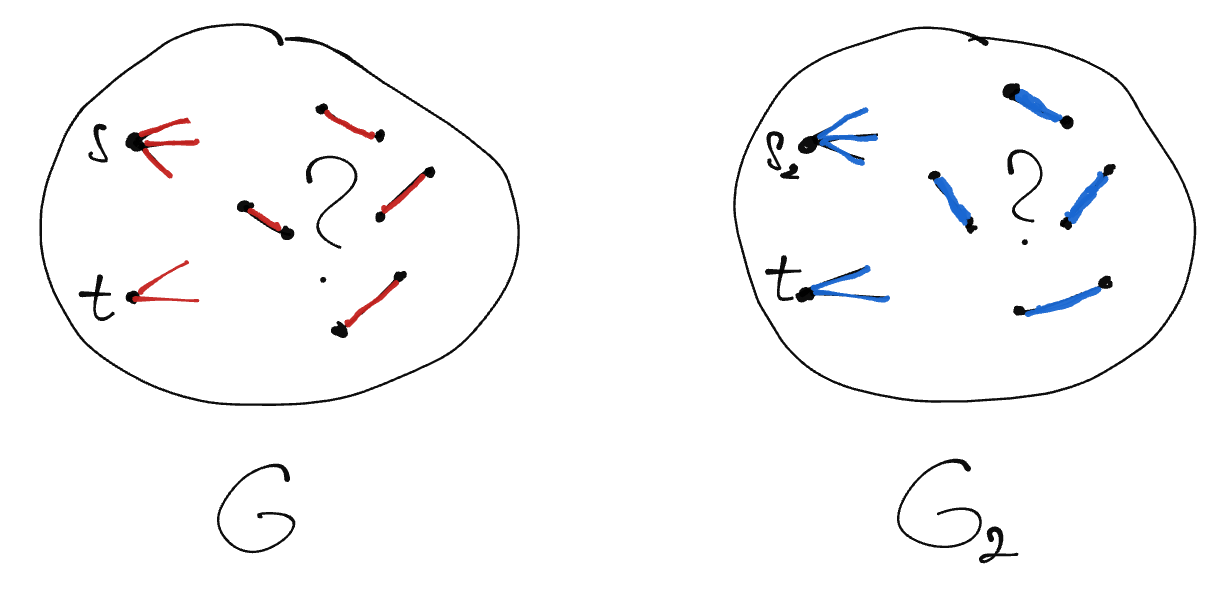
\includegraphics[width=0.9\linewidth]{./exams/2022_05_30/03/karp_2.png}
\end{center}

\begin{itemize}
    \item Finally, we will connect $s$ and $s_2$ with a red edge, while we will connect the $t$ and $t_2$ with a blue edge:
\end{itemize}

\begin{center}
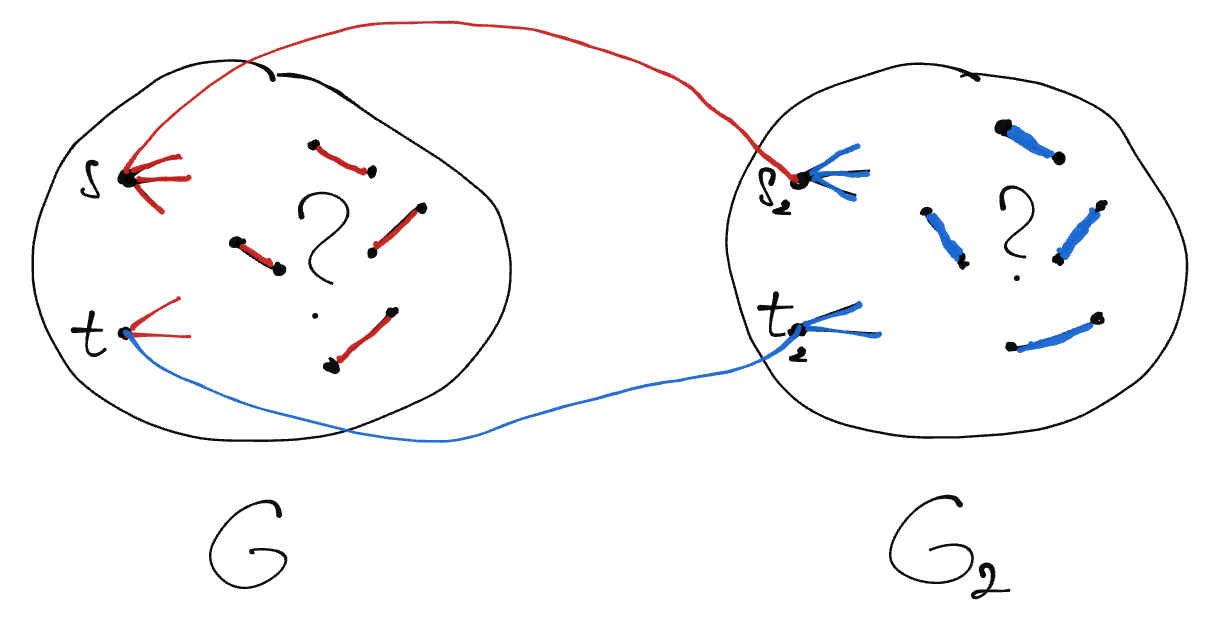
\includegraphics[width=0.9\linewidth]{./exams/2022_05_30/03/karp_3.png}
\end{center}

\begin{itemize}
    \item Now. Let's see what we have created here.
    \item If $G$ had an s-t-HAMPATH, what did that turn into?
\end{itemize}

\begin{center}
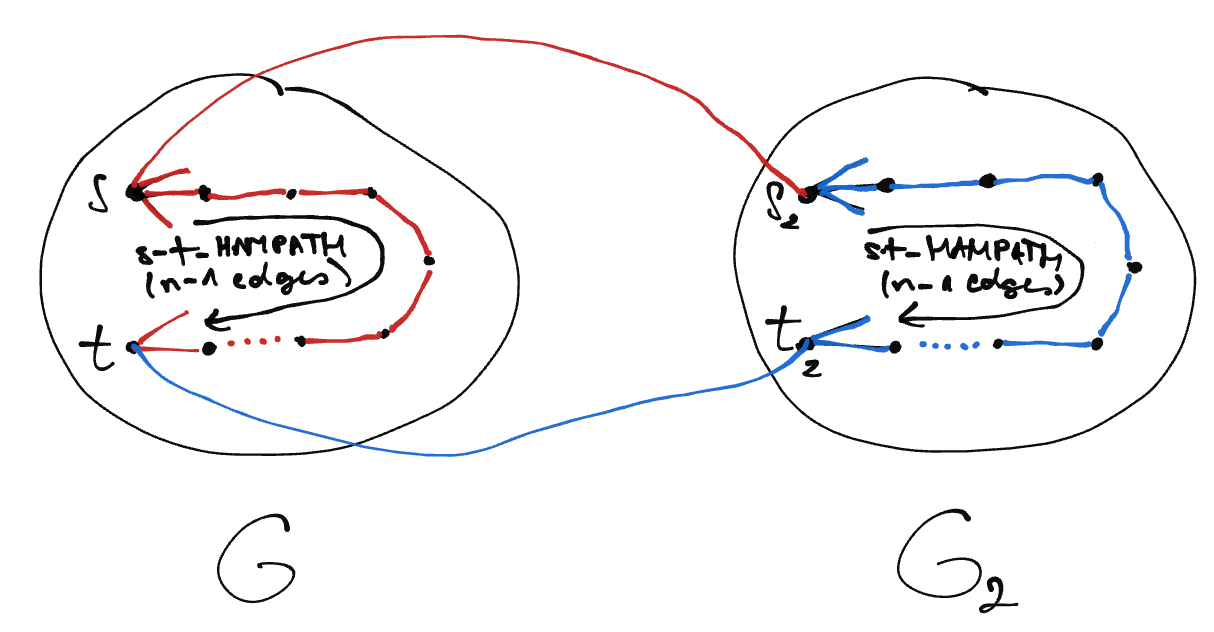
\includegraphics[width=0.9\linewidth]{./exams/2022_05_30/03/karp_where.png}
\end{center}

\begin{itemize}
    \item The s-t-HAMPATH was copied to $G_2$ as well, $G$'s s-t-HAMPATH was colored red, while $G_2$'s s-t-HAMPATH was colored blue.
    \item A Hamiltonian-cycle has emerged in this $G\cup{}G_2$ graph: Follow along the $(n-1)$ red edges, then use $s-s_2$, then follow along the $(n-1)$ blue edges, finally use the edge $t_2-t$.
    \item This is exactly the type of red-blue cycle that HAMRB says yes to! So because the original $G$ graph had an s-t-HAMPATH in it, this transformation turned that into a red/blue cycle that HAMRB says yes to (the number of the red and blue edges is the same and also the number of the total vertices in the transformed graph is $2n$.)
    \item Also, we can see that if there is no s-t-HAMPATH in the original $G$ graph, then there is no way for HAMRB to find a red/blue HAM cycle in $G\cap{}G_2$, since the only possible way to connect between $G$ and $G_2$ is to use the edges $s-s_2$ and $t-t_2$, so the only way for HAMRB to find a HAM cycle in $G\cap{}G_2$ at all, is to have $G$'s vertices lined up between $s$ and $t$ on a graph, and similarly for $G_2$ between $s_2$ and $t_2$, which is the s-t-HAMPATH we are looking for.
    \item Finally, the transformation function must also be polynomial runtime. Here we duplicated $G$, and added two more edges, which can be done in polynomial time, so we are done with the proof.
\end{itemize}

Notes:
\begin{itemize}
    \item After we have completed this proof, if someone comes up with a polynomial solver for HAMRB, what can we do with it?
    \item We can insert that into our "Karp-machine", to the missing place, which will turn it into a complete polynomial solver for s-t-HAMPATH no additional steps required!
\end{itemize}

\begin{center}
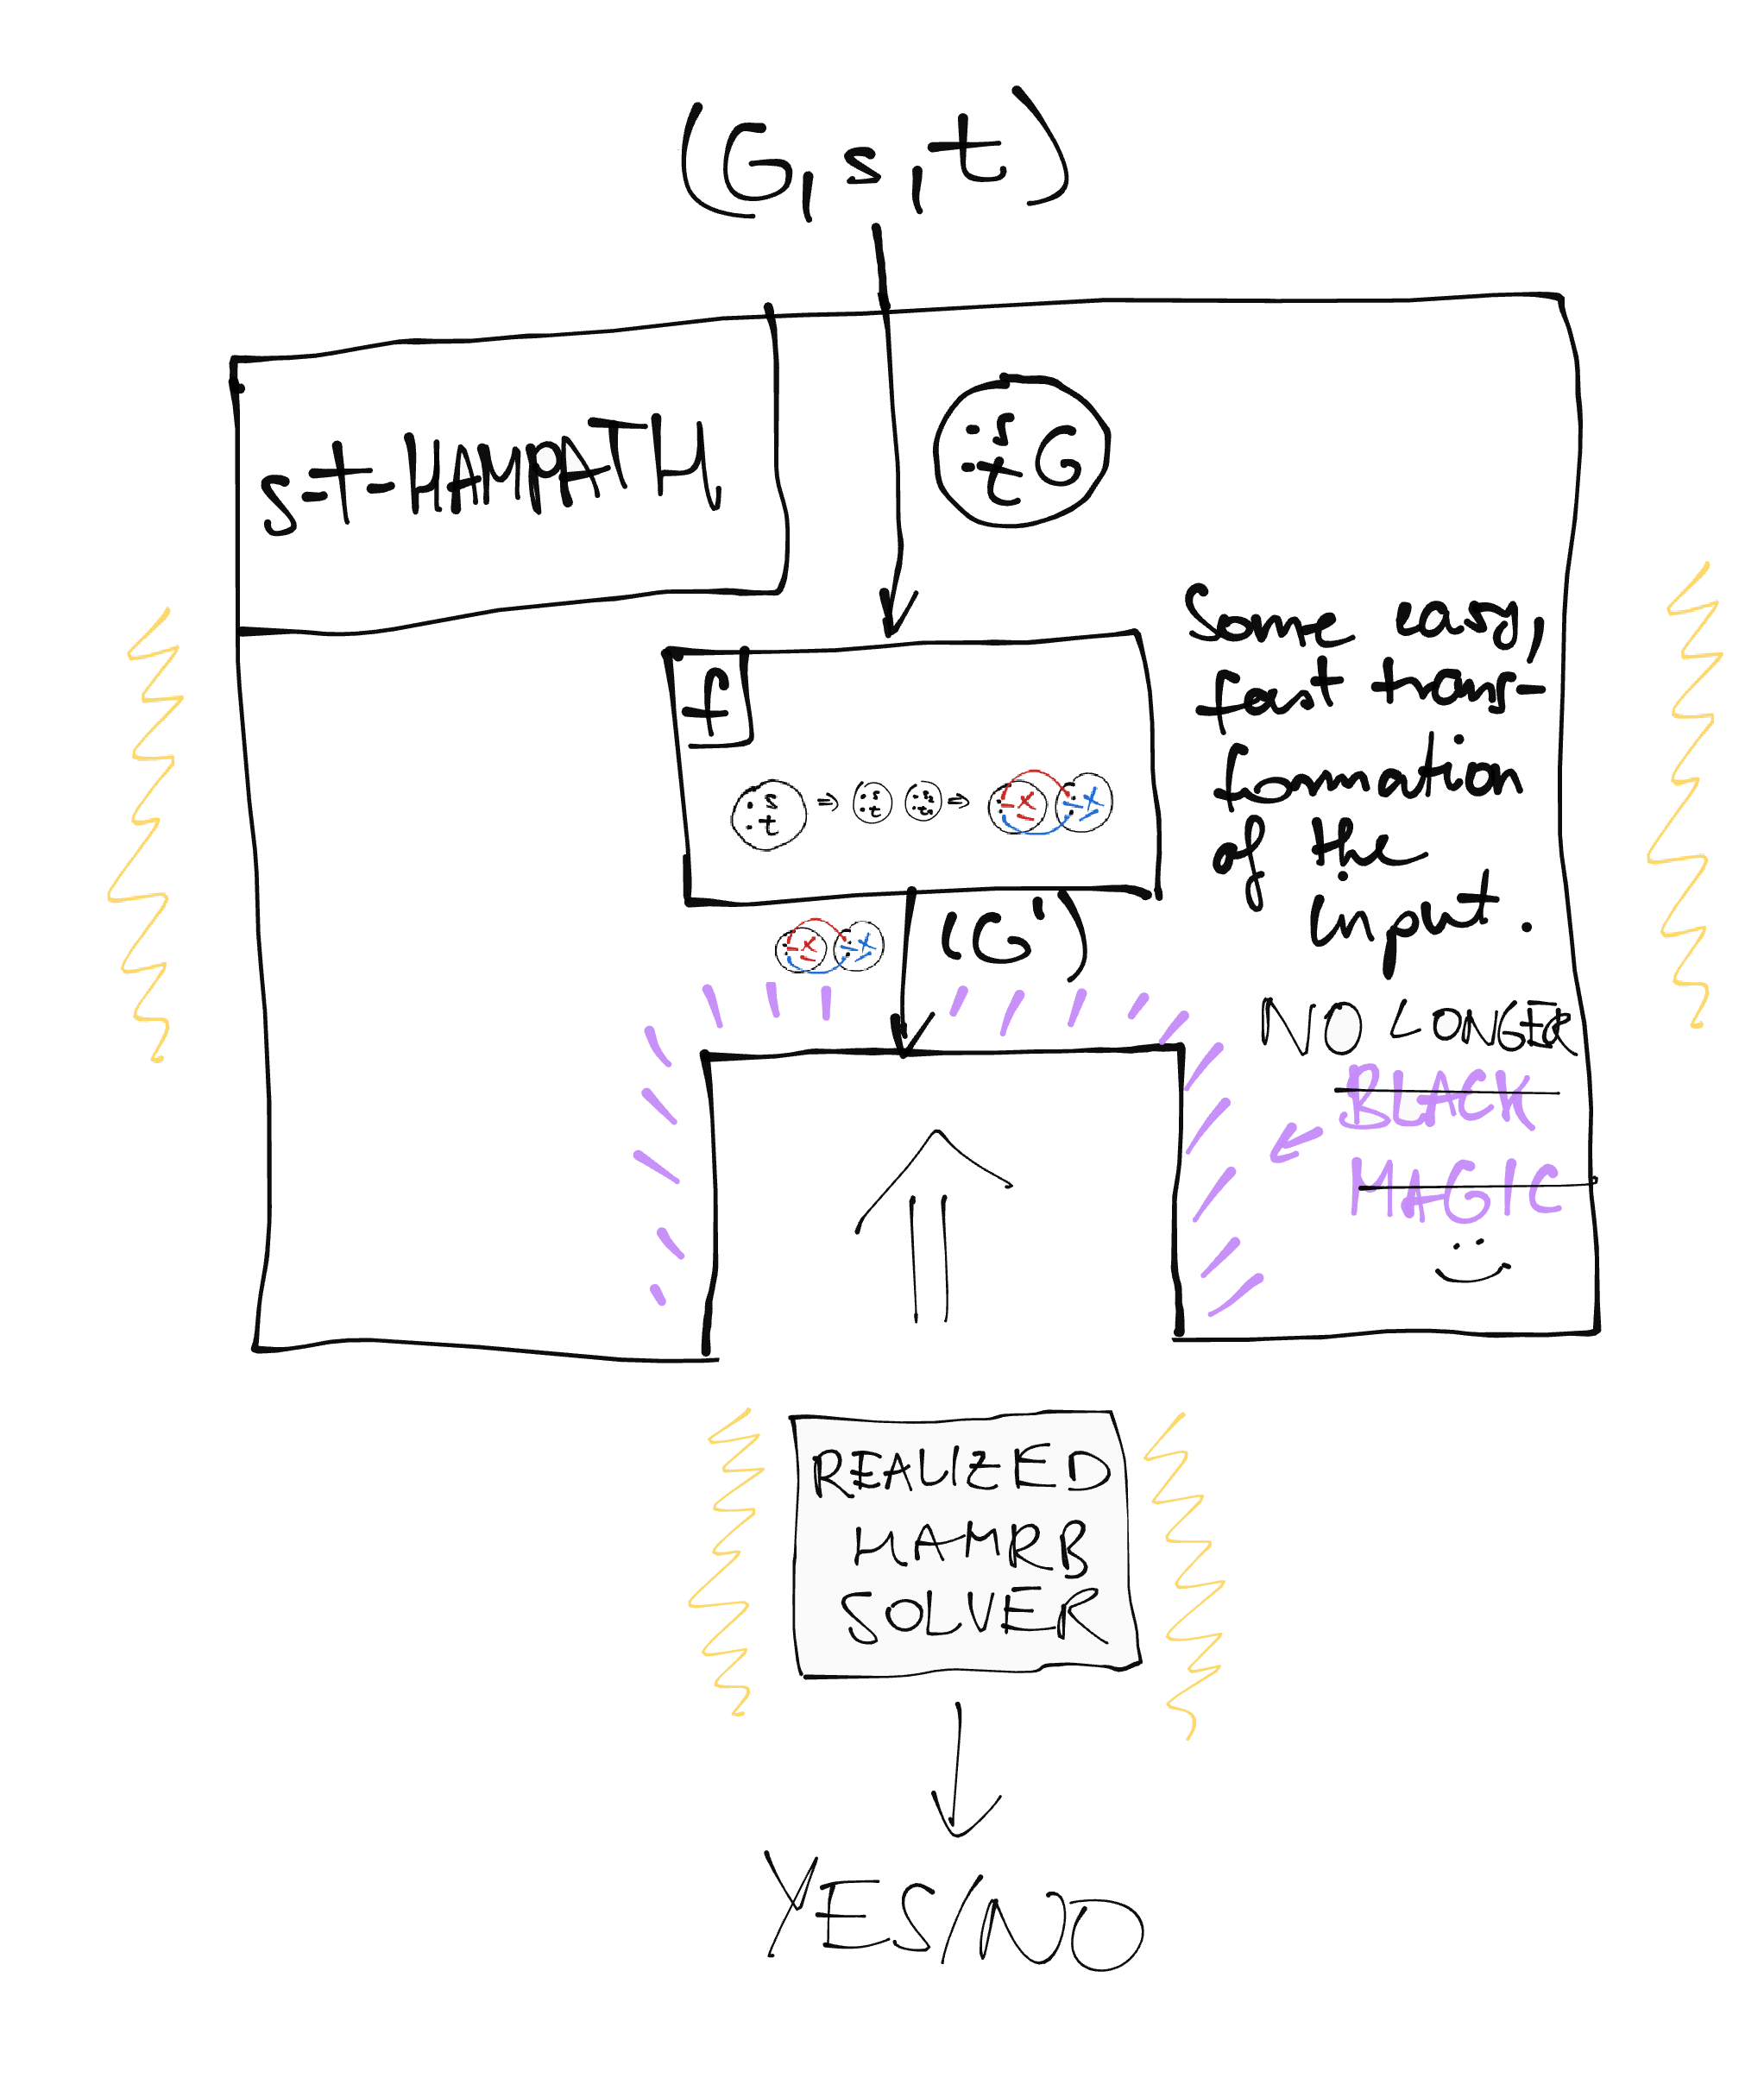
\includegraphics[width=0.9\linewidth]{./exams/2022_05_30/03/karp_insert.png}
\end{center}